\documentclass{article}
\usepackage{graphicx}

\title{Report 4 Cuda 3D processing}
\author{Le Nhu Chu Hiep}

\begin{document}

\maketitle

\section{Implementation}
\begin{itemize}
    \item Defining "grid size" and "block size" as dim3
    \item Redefining grayScale function to identify array identity from 3D index
    \item Run as normal
\end{itemize}

\section{Result}
\subsection{Text result}
\begin{verbatim}
-- Labwork 4 --
USTH ICT Master 2018, Advanced Programming for HPC.
Warming up...
Starting labwork 4
labwork 4 ellapsed 143.9ms

-- Labwork 3 --
USTH ICT Master 2018, Advanced Programming for HPC.
Warming up...
Starting labwork 3
blockSize: 32
labwork 3 ellapsed 4243.4ms
\end{verbatim}

\subsection{Figure result}
\begin{figure}
        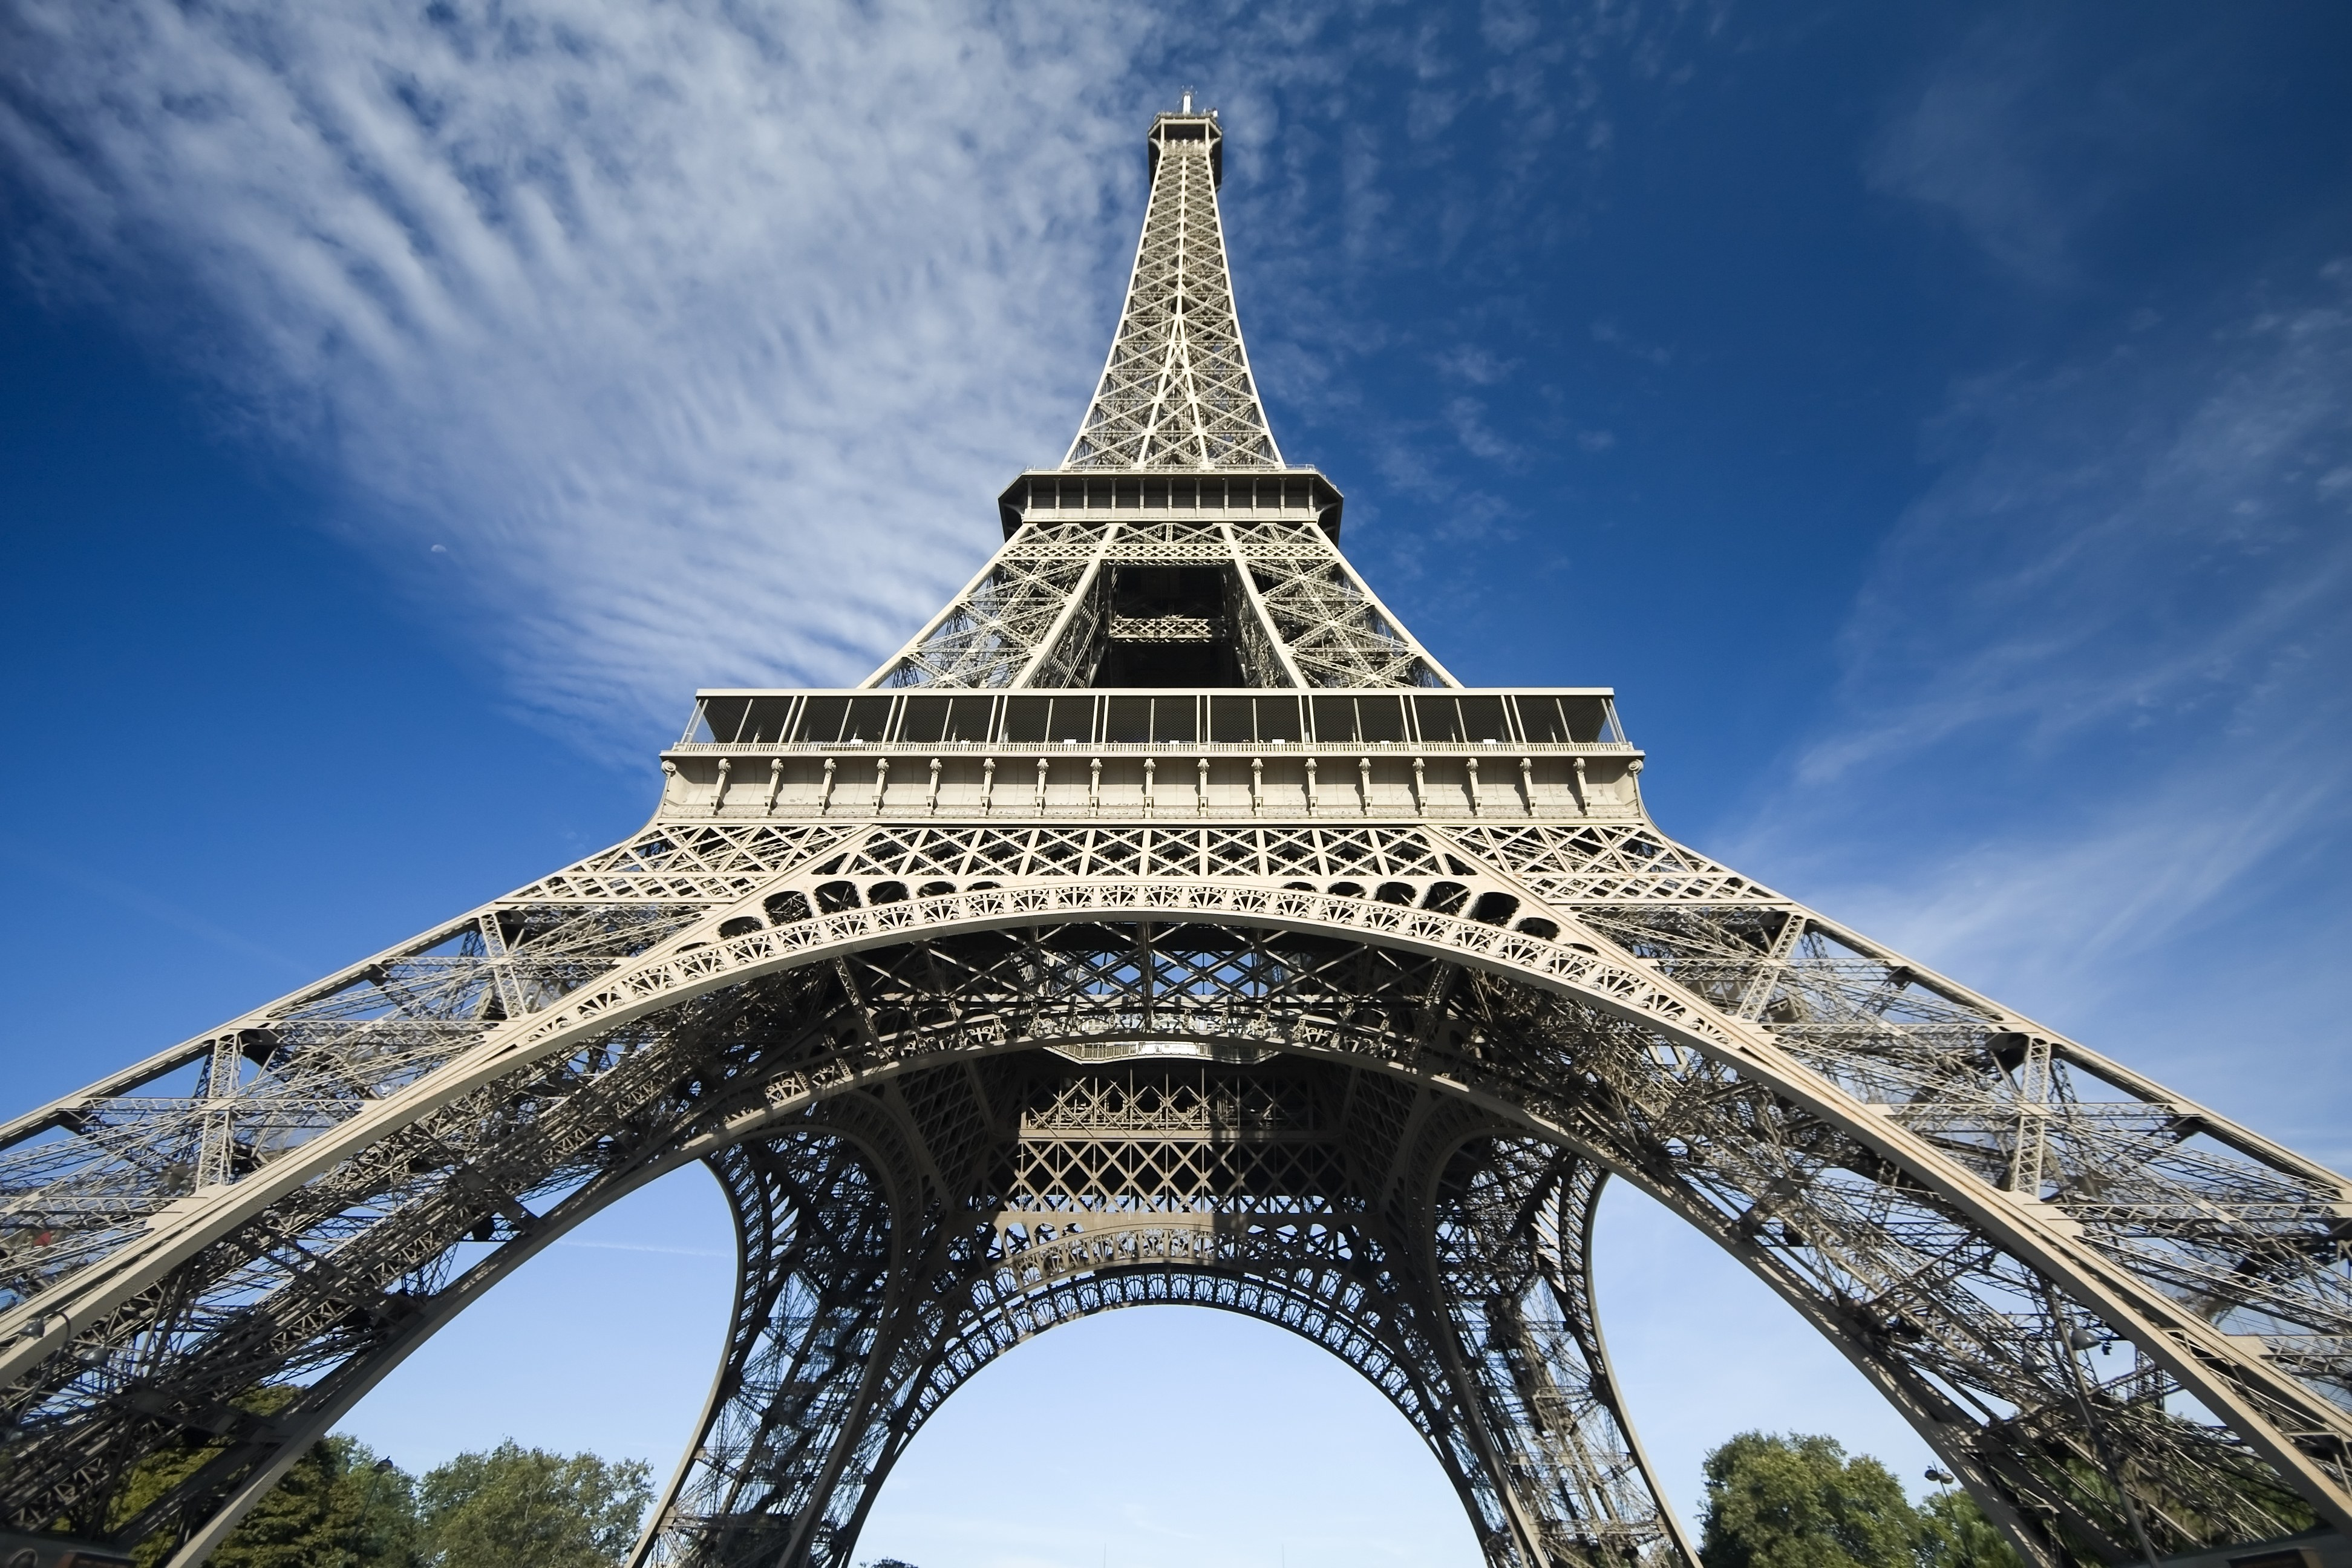
\includegraphics[width=\textwidth]{./labwork/data/eiffel.jpg}
        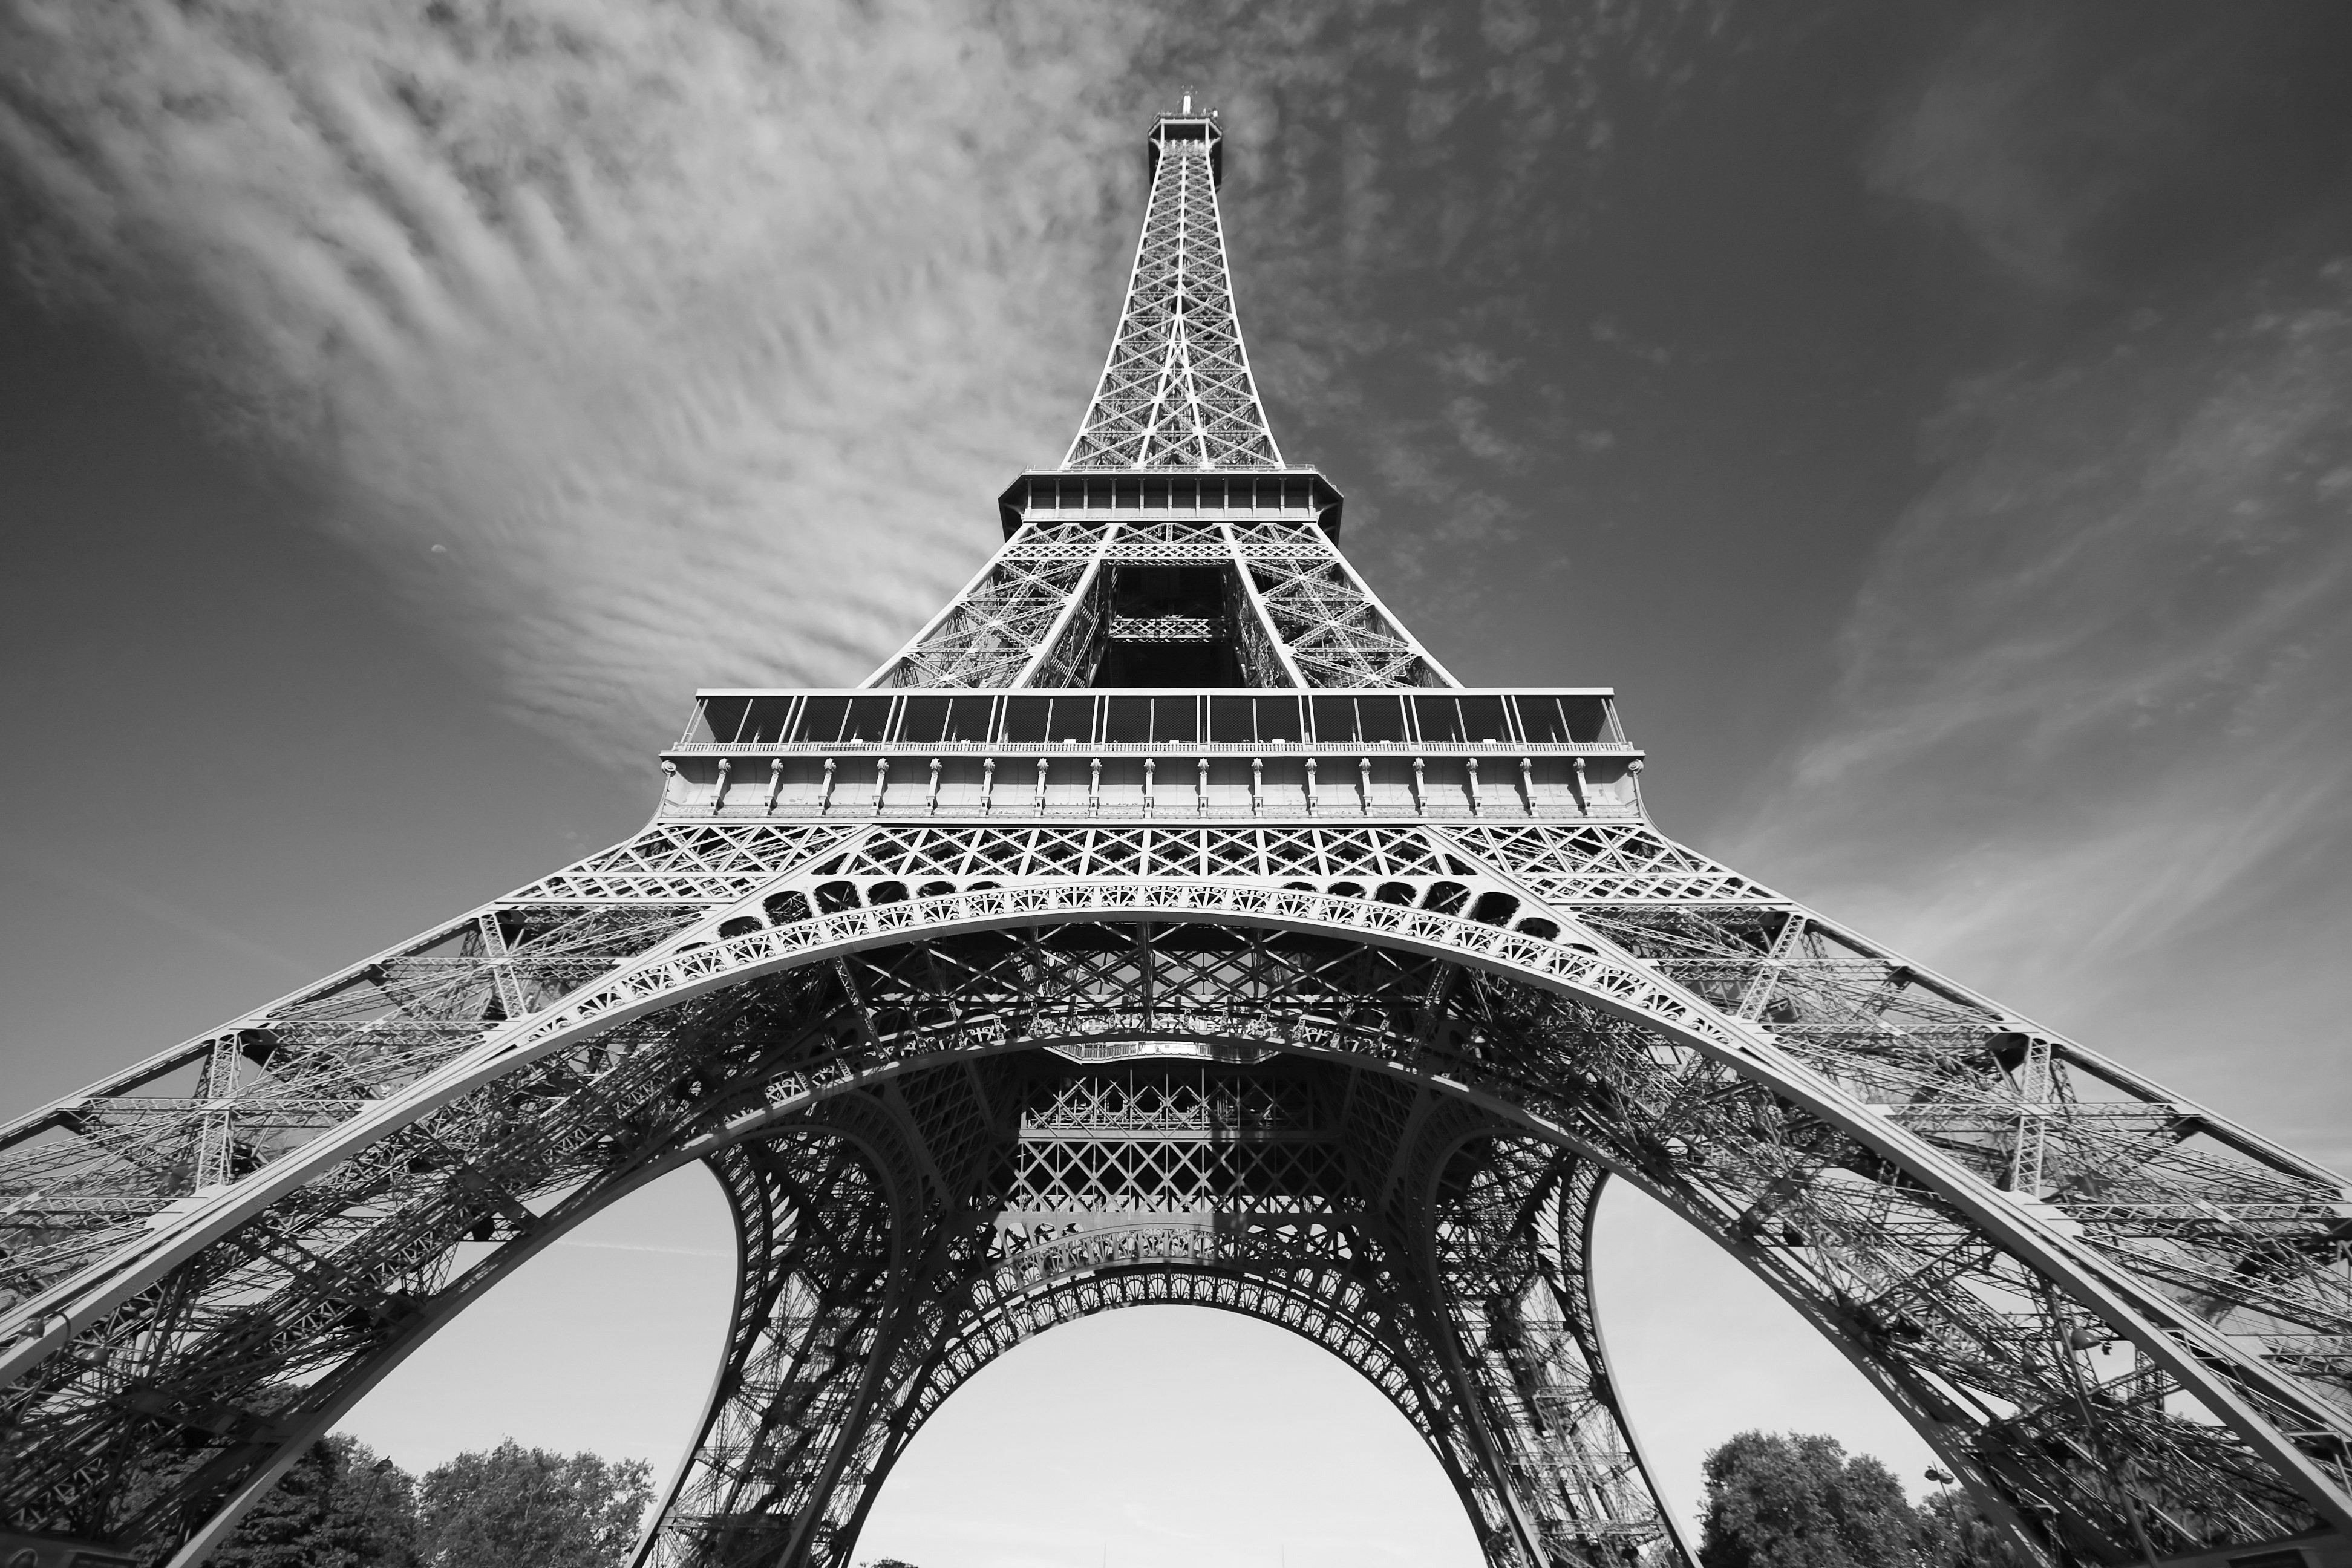
\includegraphics[width=\textwidth]{./labwork4-gpu-out.jpg}
        \caption{Eiffel picture}
\end{figure}
\end{document}
